\chapter{Multipliers}\label{ch:multipliers}

In the previous chapters, I provided robust linguistic evidence for the relevance of subatomic quantification in natural language as well as for the significant role the topological notion of integrity plays with respect to that phenomenon. I examined multiple types of partitive constructions including count explicit partitives and topology-sensitive proportional partitives. What these two types of expressions have in common is that they impose a certain constraint on how the denoted parts of objects are conceptualized. Specifically, they require the parts to constitute integrated continuous elements. On the other hand, we saw that subatomic quantification is not restricted to partitive constructions and is also attested in the adjectival domain, e.g., German and Romance adjectival half-words as well as different types of whole-adjectives. At this point, one could expect that given the amount of evidence for the relevance of part-whole structures in different types of constructions there should be quantificational expressions in natural language that are specialized for counting parts of entities. It turns out that in fact in many languages there are such expressions.\largerpage[3]  

In this chapter, I will present novel data concerning subatomic quantification in the adjectival domain. In particular, I will examine semantic properties of numerical expressions such as English \textit{double} and \textit{triple} which I will refer to as \textsc{multipliers} \citep[following][]{quirk_greenbaum_leech_svartvik1985comprehensive,huddleston_pullum2002cambridge}. In particular, I will focus mostly on Slavic multipliers exemplified by Polish \textit{podwójny}, Czech \textit{dvojitý}, Russian \textit{dvojnoj}, and Bosnian-Croatian-Serbian (BCS) \textit{dvostruki}, all `double', which all seem to have identical properties. Unlike cardinal numerals, multipliers do not count entities, but rather their particular parts. I have chosen Slavic multipliers due to their morphological complexity which suggests a rich semantic structure that is not expressed formally in a language such as English. To foreshadow, I will argue that since multipliers in Slavic are derivationally complex, they are in fact compositional. Though the distribution of multipliers is relatively broad, I will mainly concentrate on a subset of environments in which they can occur, which allows us for novel insights with respect to the phenomena discussed in this study.\footnote{Most of the data discussed in this chapter come from linguistic corpora. However, I would like to sincerely thank Mojmír Dočekal, Pavel Caha, and Markéta Ziková, Tetiana Kamyshanova, Boban Arsenijević, Kurt Erbach and Guy Tabachnick, and Viola Schmitt for confirming my intuitions concerning some of the Czech, Russian, BCS, English, and German phrases, respectively.}

\section{Significance of multipliers}\label{sec:significance-of-multipliers}\largerpage[2]

Since the early days of formal semantics \citep[starting with][]{montague1973proper} the meaning of quantificational expressions such as numerals has been constantly receiving a lot of attention. Over the last several decades, extensive and extremely important work has been done in this area leading to a number of influential theories of cardinals \citep[e.g.,][]{barwise_cooper1981generalized,scha1981distributive,landman2004indefinites,ionin_matushansky2006composition}. Nevertheless, it seems that there is still a vast territory left unchartered since natural languages exhibit multiple classes of numerical expressions that did not receive nearly as much recognition as cardinal numerals. In this chapter, I will contribute to the study of such somewhat neglected classes of quantifiers by providing evidence considering multipliers. Though such expressions are cross-linguistically common, see \ref{ex:multipliers-intro}, as for now their semantic properties are surprisingly understudied and I am not aware of any formal attempt to account for their behavior and meaning.\footnote{An exception is \citet{wagiel2020entities} on which the whole chapter is loosely based.}

\ex.\label{ex:multipliers-intro} \a. English\\
double
\b. German\\
doppelt
\b. Italian\\
doppio
\b. Lithuanian\\
dvigubas
\b. Finnish\\
kaksinkertainen
\b. Hungarian\\
dupla
\b. Mandarin\\
shu{\=a}ng

The fact that multipliers have been somewhat overlooked is even more striking given that they exhibit non-trivial quantificational behavior that differs significantly from the one observed in cardinal numerals. For instance, consider examples such as those in \ref{ex:crown-two-double}. 

\ex. English\label{ex:crown-two-double}
\a. crown\label{ex:crown}
\b. two crowns\label{ex:two-crowns}
\b. double crown\label{ex:double-crown}

The noun phrase in \ref{ex:crown} simply denotes a set of singular entities having the property of being a crown. Interestingly, although the phrase in \ref{ex:two-crowns} is true of a plurality of two entities, \ref{ex:double-crown} can only be interpreted as referring to a single individual, similarly to \ref{ex:crown}. There is, however, a crucial difference between the two expressions since \ref{ex:double-crown} seems to involve subatomic quantification. In particular, the multiplier appears to quantify over elements within the inner structure of a denoted entity. In other words, \textit{double} in \ref{ex:double-crown} restricts the denotation of the noun to only those crowns that have a particular complex form.

In the following parts of this chapter, I will discuss the distribution and semantic properties of Slavic multipliers with a special focus on Polish. I will argue that such expressions are compositional and involve quantification over objects that are conceptualized as integrated parts of integrated wholes. Furthermore, I will suggest a generalization concerning the meaning of a representative subset of the data, i.e., multiplier phrases involving concrete singular nouns, and point out some non-trivial consequences as well as discuss other types of nominals multipliers that combine with and how it relates to subatomic quantification.

\subsection{Morphological complexity of Slavic multipliers}\label{sec:morphological-complexity-of-slavic-multipliers}

Since it is widely recognized that derivational morphology in Slavic languages is particularly rich, in recent years increasing attention has been drawn to the semantics of Slavic morphologically complex numerical expressions. The research has led to a number of insightful investigations concerning such constructions in Czech \citep[e.g.,][]{docekal2012atoms,docekal2013numerals,docekal_wagiel2018event,grimm_docekal-toappear-counting}, Polish \citep[e.g.,][]{wagiel2014boys,wagiel2015sums,wagiel2020entities,wagiel2020several,wagiel-toappear-grammatical}, and Russian \citep[e.g.,][]{khrizman2015cardinal}. However, while previous research focused mainly on the impact of numeral morphology on the collective/distributive alternation with respect to different types of numerals, in this study I will examine the adjectival domain and present evidence of the significance of multipliers for subatomic quantification, i.e., quantification over cognitively salient parts of entities. In \sectref{sec:continuous-discontinuous-parts} and \sectref{sec:more-topology-sensitive-partitive-words}, we saw how formal complexity correlates with topology-sensitive semantics in partitive words in Polish. In this section, I will focus on the morphology of Polish, Czech, Russian, and BCS multipliers which unlike their English counterparts exhibit a complex derivational structure. I believe this choice of data will be instructive since it will allow us to confront multipliers with cardinals in a straightforward manner that will reveal intriguing similarities as well as differences between the two classes. 

The examined lexical items in question will be exemplified in the following sections by expressions derived from the numeral root $\sqrt{\textit{dw}}$~/~$\sqrt{\textit{dv}}$ corresponding to the number 2. Let us assume the morphological make-up of the basic cardinals and matching multipliers as in \ref{ex:cardinal-multiplier-morphology-polish}--\ref{ex:cardinal-multiplier-morphology-bcs}.\footnote{For convenience, I provide only unmarked forms for cardinals in \ref{ex:cardinal-morphology-polish}--\ref{ex:cardinal-morphology-bcs}. In a similar vein, in \ref{ex:multiplier-morphology-polish}--\ref{ex:multiplier-morphology-bcs} masculine forms represent whole declensional paradigms. For BCS in \ref{ex:multiplier-morphology-bcs}, the derivationally complex adjective \textit{dvostruki} `double' has been chosen for sake of exposition despite the fact that there is also another BCS multiplier, namely \textit{dupli} `double'. Although it seems that there is a difference in the distribution of the two forms, I assume that there is no relevant semantic distinction between them with respect to the phenomena discussed here.}

\ex. Polish\label{ex:cardinal-multiplier-morphology-polish}
\a. dw-a\\
numeral.root-inflectional.marker\\
`two'\label{ex:cardinal-morphology-polish}
\b. po$\rangle$dw-ój$\langle$n-y\\
circumfix$\rangle$numeral.root-non.card.stem$\langle$circumfix-infl.marker\\
`double'\label{ex:multiplier-morphology-polish}

\ex. Czech\label{ex:cardinal-multiplier-morphology-czech}
\a. dv-a\\
numeral.root-inflectional.marker\\
`two'\label{ex:cardinal-morphology-czech}
\b. dv-oj-it-ý\\
numeral.root-non.cardinal.stem-deriv.suffix-infl.marker\\
`double'\label{ex:multiplier-morphology-czech}

\ex. Russian\label{ex:cardinal-multiplier-morphology-russian}
\a. dv-a\\
numeral.root-inflectional.marker\\
`two'\label{ex:cardinal-morphology-russian}
\b. dv-oj-n-oj\\
numeral.root-non.cardinal.stem-deriv.suffix-infl.marker\\
`double'\label{ex:multiplier-morphology-russian}

\ex. BCS\label{ex:cardinal-multiplier-morphology-bcs}
\a. dv-a\label{ex:cardinal-morphology-bcs}\\
numeral.root-inflectional.marker\\
`two'
\b. dv-o-struk-i\\
numeral.root-non.cardinal.stem-deriv.suffix-infl.marker\\
`double'\label{ex:multiplier-morphology-bcs}

As can be witnessed in the morpheme orderings in \ref{ex:multiplier-morphology-polish}--\ref{ex:multiplier-morphology-bcs}, all the multipliers in question consist of numeral roots shared with corresponding cardinals and some additional morphology including the affixes \textit{po}$\rangle$\dots$\langle$\textit{n-}/\textit{-it-}/\textit{-n-}/\textit{-struk-} and the morphemes \textit{-ój-}/\textit{-oj-}/\textit{-o-}, which mark a non-cardinal stem as well as inflectional markers. Notice that the morphemes \textit{-ój-}/\textit{-oj-}/\textit{-o-} appear in multipliers derived from numeral roots referring to the numbers 2--3. In multipliers derived from roots referring to the number 4, the suffix \textit{-ór-}/\textit{-er-}/\textit{-oro-} occurs instead, e.g., Polish \textit{po}$\rangle$\textit{czw-ór}$\langle$\textit{n-y}, Czech \textit{čtv-er-n-ý}, Russian\textit{ četv-er-n-oj}, and BCS \textit{četv-oro-stuk-i}, all meaning `quadruple'.

In general, Slavic multipliers exhibit adjectival morphology and agree with modified nouns in case, number, and gender, as in \ref{ex:multiplier-agreement-polish}. 

\ex. Polish\label{ex:multiplier-agreement-polish}
\bg.[] Ta podwójna szyba się stłukła.\\
this\textsc{.nom.sg.f} double\textsc{.nom.sg.f} glass\textsc{.nom.sg.f} \textsc{refl} broke\textsc{.sg.f}\\
`This double glazing broke.'

I will refer to the derivational circumfix \textit{po}$\rangle$\dots$\langle$\textit{n-} in Polish and the suffixes \textit{-it-}, \mbox{\textit{-n-},} and \textit{-struk-} in Czech, Russian, and BCS, respectively, as multiplicative morphemes. Moreover, I will assume here that inflectional markers and morphemes constituting non-cardinal stems have no contribution to the semantics of multipliers. Therefore, in the analysis to come I will focus only on the interaction between numeral roots and multiplicative morphemes.

An approach neglecting the semantic role of some of the examined morphemes in composition might seem in fact a considerable simplification since affixes marking non-cardinal stems are attested not only in multipliers, but also in a variety of other numerical expressions. For instance, consider Polish denumeral group nouns such as \textit{dwójka} `(group of) two', derived numerals presupposing that a plurality is heterogeneous with respect to the natural gender of referents such as \textit{dwoje} `two (one male and one female)', taxonomic numerals like \textit{dwojaki} or \textit{dwoisty}, both `twofold', as well as denumeral verbs such as \textit{podwoić} `to double'.\footnote{See \citet{wagiel2014boys,wagiel2015sums} for a discussion and possible analysis of expressions such as \textit{dwójka} and \textit{dwoje}. Notice also that \textit{-ój-}, \textit{-oj-}, and \textit{-oi}- are allomorphs.} At first blush, it seems appealing to assume that the appearance of non-cardinal stem markers in all the above cases is non-coincidental from a semantic point of view. Therefore, an alternative approach could assign, e.g., Polish \textit{-ój-}/\textit{-oj-}/\textit{-oi-} a meaning general enough to cover the whole variety of considered expressions, i.e., an underspecified operation on numbers that is different from the one employed in cardinals. Nevertheless, in this study I will remain agnostic with respect to that possibility. Instead, I will assume that the discussed markers are semantically vacuous and that their sole function is purely structural, specifically they simply form stems. For the sake of simplicity I will also ignore all the intricacies related to the semantics of gender as well as its relationship with quantification \citep[see, e.g.,][]{arsenijevic2017gender,fassi_fehri2016semantic,fassi_fehri2018constructing,wagiel-toappear-grammatical} and the role of inflectional markers in coding such an interaction.

\subsection{Subatomic quantifiers}\label{sec:subatomic-quantifiers}

In the previous section, we saw that in Slavic the morphological make-up of multipliers resembles that of cardinals with the crucial difference that the former consistently involve more structure. Let us now consider the meaning of phrases in which multipliers modify a noun. I will start with the set of examples in \ref{ex:double-crown-polish}--\ref{ex:double-crown-bcs}, which are semantically analogous and equivalent to the English phrase in \ref{ex:double-crown}. 

\ex. Polish (NCP)\label{ex:double-crown-polish}
\bg.[] podwójna korona\\
double\textsc{.sg.f} crown\textsc{.f}\\
`double crown'

\ex. Czech (CNC)\label{ex:double-crown-czech}
\bg.[] dvojitá	koruna\\
double\textsc{.sg.f} crown\textsc{.f}\\
`double crown'

\ex. Russian (RNC)\label{ex:double-crown-russian}
\bg.[] dvojnaja	korona\\
double\textsc{.sg.f} crown\textsc{.f}\\
`double crown'

\ex. BCS (CrNC)\label{ex:double-crown-bcs}
\bg.[] dvostruka kruna\\
double\textsc{.sg.f} crown\textsc{.f}\\
`double crown'

The examples provided above will be considered as illustrative since they are all attested in representative Slavic text corpora such as the National Corpus of Polish (NCP) \citep{przepiorkowski_et-al2012narodowy}, the Czech National Corpus (CNC) \citep{kren_et-al2020syn2020}, the Russian National Corpus (RNC) \citep{apresjan_et-al2006syntactically}, and the Croatian National Corpus (CrNC) \citep{tadic2009new}.\footnote{NCP: \url{http://nkjp.pl/}, CNC: \url{https://www.korpus.cz/}, RNC: \url{https://ruscorpora.ru/new/}, CrnC: \url{http://filip.ffzg.hr/cgi-bin/run.cgi/first_form}.} Furthermore, the Polish noun \textit{korona} `crown' ranks at the 13th place on the list of collocation candidates within two-words collocations for the form \textit{podwójna} `double' in the balanced sample of the National Corpus of Polish whereas the Czech noun \textit{koruna} `crown' ranks at the 7th place for the form \textit{dvojitá} `double' in a corresponding Czech sample in the Czech National Corpus. Moreover, the example is of historical relevance since it resembles the famous case of the complex papal crown discussed in the philosophical literature \citep[see][p. 70]{wiggins1980sameness}, which I will also briefly address below.

As already mentioned, noun phrases such as those in \ref{ex:double-crown-polish}--\ref{ex:double-crown-bcs} denote sets of singular (and not plural) entities despite the fact that in the morphological make-up of multipliers modifying a noun there are numeral roots which involve reference to the number 2. Given the classical perspective on the meaning of numerals, at first sight this fact might appear somewhat puzzling. Nevertheless, it seems clear that in all the multiplier examples discussed in this chapter quantification is involved albeit it is not quantification over wholes. To illustrate this claim, let us consider the historical example in \ref{ex:pschent-entailment}.\footnote{In the following part of this section, the phenomena will be discussed mainly on the basis of Polish examples. However, the generalizations are intended to hold for every language in question.} 

\ex. Polish\label{ex:pschent-entailment}
\ag. \jdg{} Pszent to podwójna korona.\\
{} Pschent this double crown\\
`The Pschent is a double crown.'\label{ex:pschent-entailment-double-crown}
\bg. \jdg{$\models$} Pszent składa się z dwóch części.\\
 {} Pschent consists \textsc{refl} from two\textsc{.gen} parts\textsc{.gen}\\
`The Pschent consists of two parts.'\label{ex:pschent-entailment-two-parts}

The sentence in \ref{ex:pschent-entailment-double-crown} indicates a complex inner structure of the Pschent, and thus entails the sentence in \ref{ex:pschent-entailment-two-parts}. If it is true of an object that it is a double crown, it has to be a crown and it has to consist of (at least) two elements.

However, it is not sufficient that the object referred to by the noun \textit{Pszent} consists of any two elements since it is not the case that every crown consisting of two parts is a double crown. Rather, the two relevant elements need to have a particular property, i.e., a property comparable to the property of the whole. In other words, a double crown consists of two parts which can be considered crowns themselves. For instance, a reader familiar with ancient history will recognize the Pschent as a crown worn by rulers of Ancient Egypt. Historically, as demonstrated in \figref{fig:pschent} the Pschent combined two parts, i.e., the Red Deshret Crown of Lower Egypt, see \figref{fig:deshret}, and the White Hedjet Crown of Upper Egypt, see \figref{fig:hedjet}.\footnote{The pictures in \figref{fig:pschent}--\ref{fig:hedjet} are based on the work by fi:Käyttäjä:kompak shared on Wikimedia Commons under the CC-BY-SA 2.5 license. Sources: \url{https://commons.wikimedia.org/wiki/File:Pschent2.svg}, \url{https://commons.wikimedia.org/wiki/File:Deshret.svg}, and \url{https://commons.wikimedia.org/wiki/File:Hedjet.svg}.} Its design represented the pharaoh's power over all of the unified kingdom. Due to the discussed features of the relevant parts of the Pschent, one could say it is a two-in-one crown.

\begin{figure}[h!]
\begin{floatrow}
\captionsetup{margin=.05\linewidth}
\ffigbox[.33\textwidth]{\caption{Pschent}\label{fig:pschent}}
        {
\includegraphics[scale=0.14]{figures/pschent.png}}
\ffigbox[.33\textwidth]{\caption{Deshret}\label{fig:deshret}}
        {
\includegraphics[scale=0.07]{figures/deshret.png}}
\ffigbox[.33\textwidth]{\caption{Hedjet}\label{fig:hedjet}}
        {
\includegraphics[scale=0.12]{figures/hedjet.png}}
\end{floatrow}
\end{figure}

Note that there is only one cut that divides the Pschent into the Deshret and Hedjet and this characteristic can be generalized to any hypothetical double crown. In other words, not every part of a double crown is a crown itself. On the contrary, in this and similar cases within the set of all the parts of a whole there are exactly two parts of which a property comparable to the property of the whole holds. Therefore, the semantics of Slavic predicates such as those in \ref{ex:double-crown-polish}--\ref{ex:double-crown-bcs} and others corresponding to the English phrase \textit{double crown} does not involve the property of divisive reference which is sometimes assumed to hold for mass nouns \citep[e.g.,][]{cheng1973comments}.\footnote{I do not share this view. For an overview of the problems related to treating divisive reference as the hallmark of mass terms see, e.g., \citet[pp. 111--119]{grimm2012number}.} Notice also that the referents of multiplier phrases differ from things designated by nouns like \textit{twig}, \textit{rock}, and \textit{fence}. Though such entities also involve parts that have the property of a whole, e.g., parts of a twig are also twigs and parts of a rock are also rocks \citep[e.g.,]{zucchi_white2001twigs,rothstein2010counting}, the crucial distinction lies in the level of the arbitrariness of subdivisions. While objects in the extensions of \textit{twig}-like expressions can be partitioned in an arbitrary manner and the resulting parts will still have the property of a whole (assuming some level of granularity) as long as they form continuous segments, complex individuals denoted by multiplier phrases typically require a very specific subdivision in order to identify the salient parts. This property makes them on a par with the already mentioned example of the papal tiara \citep[see][p. 70]{wiggins1980sameness} which is a complex object constituting a triple crown. What I believe to be the signature property of such individuals is that they are simultaneously perceived as one integrated entity and as a configuration of parts that could be considered independent objects in their own rights.

At this point, one might object that the double crown example is somewhat fancy and does not really reveal the meaning of multipliers. However, the characteristic described above is also valid for many other examples including nouns ranked relatively high as collocation candidates in the NCP. For instance, consider \ref{ex:double-examples}.

\ex. Polish (NCP)\label{ex:double-examples}
\ag. podwójne drzwi\\
double\textsc{.pl} doors\\
`double door'\label{ex:double-door}
\bg. podwójny garaż\\
double\textsc{.sg.m} garage\textsc{.m}\\
`double garage'\label{ex:double-garage}

As for \ref{ex:double-door}, the noun \textit{drzwi} `door' ranks at the 23rd place on the NCP collocation list for the non-virile/neuter form \textit{podwójne}.\footnote{Notice that in Polish the noun \textit{drzwi} `door' is a plurale tantum.} An object referred to by the phrase is a door made of two independently moving leafs, i.e., entities that could be perceived as self-sufficient doors. Likewise, a double garage denoted by the expression in \ref{ex:double-garage} can be a building with two entrances leading to separate parking spaces.\footnote{Notice, however, that similarly to the English phrase \textit{double garage} \ref{ex:double-garage} can also mean simply a garage that is big enough to fit two cars.} Again, it appears that the structure of the entity in question involves parts that can be considered as having a property similar to the property of the whole. 

The same way of thinking about multiplier phrases also applies to examples that at first blush appear to be less obvious than those discussed above. For instance, Polish multipliers frequently occur in constructions such as those provided in \ref{ex:double-examples-vague}.\largerpage

\ex. Polish (NCP)\label{ex:double-examples-vague}
\ag. podwójna warstwa\\
double\textsc{.sg.f} layer\textsc{.f}\\
`double layer'\label{ex:double-layer}
\bg. podwójna powłoka\\
double\textsc{.sg.f} coating\textsc{.f}\\
`double coating'\label{ex:double-coating}

The intuitions about frequencies are corroborated by the fact that, e.g., the noun \textit{warstwa} `layer' ranks at the 7th place on the NCP collocation list for the feminine form \textit{podwójna}. At first sight, it seems that expressions such as \ref{ex:double-layer} and \ref{ex:double-coating} refer to homogeneous entities and as such do not designate objects involving a complex structure. However, under closer inspection it turns out that even in these cases division into parts is not arbitrary. Specifically, a double layer is normally taken to be a layer consisting of two layers merged together. Since layers are flat entities spread over some surface, only a cut alongside a certain plane can divide the two parts constituting an entity denoted by the phrase in \ref{ex:double-layer}. Similarly, the expression in \ref{ex:double-coating} designates an entity whose structure can be partitioned only in a particular manner in order to separate the salient parts. Intuitively, a double coating consists of two parts that themselves are coverings applied to the surface of some object.

Certainly, examples such as those in \ref{ex:double-crown-polish}--\ref{ex:double-crown-bcs} and \ref{ex:double-examples}--\ref{ex:double-examples-vague} do not exhaust the combinatorial potential of Slavic multipliers and some more problematic cases will be discussed subsequently in \sectref{sec:less-obvious-cases}. Nevertheless, the data discussed above indicate that at least a subset of constructions involving multipliers indicates clear cases of subatomic quantification. Noun phrases such as those in \ref{ex:double-crown-polish}--\ref{ex:double-crown-bcs} and \ref{ex:double-examples}--\ref{ex:double-examples-vague} denote sets of things conceptualized as singular objects with a complex inner structure. The role of multipliers in the discussed constructions is to quantify over particular parts of such structures, i.e., parts that have a property comparable to the property of the whole. I will refer to such elements as self-sufficient parts. However, before we turn our attention to some less obvious examples and see how far the generalization proposed above can get us, let us briefly examine to what extent the described semantic properties are representative for multiplier phrases in general.

\subsection{Cross-linguistic similarities}\label{sec:cross-linguistic-similarities}

In this section, I will discuss corpus-based evidence suggesting that the semantic behavior of multipliers discussed in the previous section is not a Slavic idiosyncrasy but it is actually widespread in languages such as English and German. In particular, I will inspect a number of phrases mostly involving some of the most frequent collocates of \textit{double} as specified by the Corpus of Contemporary American English (COCA) \citep{davies2009coca} and supplement them with German equivalents found in the German Reference Corpus (GRC) \citep{kupietz_keibel2009mannheim}.\footnote{COCA: \url{https://www.english-corpora.org/coca/}, GRC: \url{https://www.ids-mannheim.de/digspra/kl/projekte/korpora/}.} This brief investigation will both provide a slightly broader cross-linguistic perspective and prepare the ground for a discussion of more problematic cases in \sectref{sec:less-obvious-cases}.

Let us start with the English phrases in \ref{ex:double-coca-self-sufficient}.

\ex. English (COCA)\label{ex:double-coca-self-sufficient}
\a. double bracket\label{ex:double-coca-self-sufficient-bracket}
\b. double sink\label{ex:double-coca-self-sufficient-sink}
\b. double oven\label{ex:double-coca-self-sufficient-oven}
\b. double knot\label{ex:double-coca-self-sufficient-knot}

The expression in \ref{ex:double-coca-self-sufficient-bracket} is a somewhat metalinguistic example. Specifically, the symbol $\llbracket\dots\rrbracket$ used to indicate the semantic evaluation function every formal semanticist knows so well, is referred to by the pluralized phrase in \ref{ex:double-coca-self-sufficient-bracket}, i.e., \textit{double brackets}. The structure of the entity is such that each of the two parts of the, say, opening bracket can be considered a bracket itself. However, since they are spatially arranged in such a way that they form an integrated object perceived as one, under ordinary circumstances it would be rather awkward to refer to a double bracket as \textit{two brackets}. An analogous effect can be observed with respect to the meaning of the phrase in \ref{ex:double-coca-self-sufficient-sink} which refers to a basin designed in such a way that it includes two parts each of which is a sink itself. Similarly, \ref{ex:double-coca-self-sufficient-oven} is true of a cooking device that consists of two merged ovens, i.e., two parts that have a property comparable with the property of the whole. The expression \ref{ex:double-coca-self-sufficient-knot} refers to a knot wound twice which typically results in an object consisting of two recognizable parts that are knots themselves. 

Other examples of the discussed sort involve relatively frequent multiplier phrases such as those in \ref{ex:double-coca-self-sufficient-more}. 

\ex. English (COCA)\label{ex:double-coca-self-sufficient-more}
\a. double staircase\label{ex:double-coca-self-sufficient-more-staircase}
\b. double tomb\label{ex:double-coca-self-sufficient-more-tomb}
\b. double canoe\label{ex:double-coca-self-sufficient-more-canoe}
\b. double flute\label{ex:double-coca-self-sufficient-more-flute}
\b. double needle\label{ex:double-coca-self-sufficient-more-needle}
\b. double chin\label{ex:double-coca-self-sufficient-more-chin}

Each of the expressions provided above refers to an entity perceived as a complex object involving two salient parts with a property comparable to the one of the whole. Specifically, \ref{ex:double-coca-self-sufficient-more-staircase} and \ref{ex:double-coca-self-sufficient-more-tomb} denote a staircase consisting of two connected staircases and a tomb built in such a way that it comprises two tombs in one structure, respectively. Analogously, the phrases in \ref{ex:double-coca-self-sufficient-more-canoe}--\ref{ex:double-coca-self-sufficient-more-needle} designate entities conceptualized as one object consisting of two merged individuals in their own right. Finally, the frequent expression in \ref{ex:double-coca-self-sufficient-more-chin} refers to a body part that due to the excessive amount of fat or skin looks as if it were a two-layered chin.

In parallel to phrases such as \ref{ex:double-examples-vague}, the COCA provides examples of homogeneous entities involving self-sufficient parts, see \ref{ex:double-coca-vague}. The same observations I have discussed with respect to the Polish data also apply to the English expressions.

\ex. English (COCA)\label{ex:double-coca-vague}
\a. double layer\label{ex:double-coca-vague-layer}
\b. double glazing\label{ex:double-coca-vague-glazing}
\b. double stitching\label{ex:double-coca-vague-stitching}

Sometimes, parts of an individual denoted by a multiplier phrase are not actually connected but remain in such proximity that they are perceived as forming one complex entity. For instance, the phrases in \ref{ex:double-coca-self-sufficient-close-rainbow} and \ref{ex:double-coca-self-sufficient-close-star} refer to close-set pairs of meteorological and astronomical objects, respectively. In such cases, the perceived distance between individual rainbows and stars is considered so small that a pair is conceptualized as a complex entity consisting of two parts each of which has a property comparable to the one of the whole. Similar examples include, e.g., \textit{double nebula} and \textit{double cluster} which also refer to astronomical objects perceived as complex dual entities.

\ex. English (COCA)\label{ex:double-coca-self-sufficient-close}
\a. double rainbow\label{ex:double-coca-self-sufficient-close-rainbow}
\b. double star\label{ex:double-coca-self-sufficient-close-star}

The results of several quick searches in the German Reference Corpus (GRC) consulted with native speakers demonstrate that the reported effects are also attested in German. The phrases in \ref{ex:multipliers-grc} exemplify different types of referents of multiplier phrases including homogeneous entities, see \ref{ex:multipliers-grc-glazing}, and phenomena perceived as wholes consisting of similar objects remaining in relative proximity, see \ref{ex:multipliers-grc-rainbow}.\footnote{In fact, German distinguishes between two distinct, though morphologically related, multiplier expressions, e.g., adjectival \textit{doppelt} and prefixal \textit{Doppel-}. Though it seems that their distribution differs, for the sake of brevity I will not examine the alternation here and leave such an investigation for future research.}

\ex. German (GRC)\label{ex:multipliers-grc}
\ag. Doppelkrone\\
double.crown\\
`double crown'\label{ex:multipliers-grc-crown}
\bg. Doppelverglasung\\
double.glazing\\
`double glazing'\label{ex:multipliers-grc-glazing}
\bg. Doppelregenbogen\\
double.rainbow\\
`double rainbow'\label{ex:multipliers-grc-rainbow}

The quick overview of some of the frequent contexts multipliers appear in shows that the double crown example discussed in \sectref{sec:subatomic-quantifiers} is not some extravagant case. Rather, it represents common semantic behavior of multipliers. I conclude that the English and German evidence based on the collocation list from the COCA and searches in the GRC suggests that the pattern is robust. 

\subsection{Multipliers as degree modifiers}\label{sec:multipliers-as-degree-modifiers}

Briefly, I will return to the data both from Slavic and English to examine somewhat more problematic examples. Nonetheless, before I move on to the discussion of cases where at least at first sight intuitions concerning the subatomic structure of entities denoted by multiplier phrases are not that clear, let us discuss yet another use of the expressions in question. In English, multipliers can be used as predeterminer modifiers, i.e., external modifiers of the whole DP occurring before the central determiner such as the definite article (see, e.g., \citealt[pp. 257--258]{quirk_greenbaum_leech_svartvik1985comprehensive}; \citealt[pp. 433--436]{huddleston_pullum2002cambridge}).\footnote{Actually, the term predeterminer modifier is used only by \citeauthor{huddleston_pullum2002cambridge}. \citeauthor{quirk_greenbaum_leech_svartvik1985comprehensive} use the term predeterminer instead.} Examples of such uses are given in \ref{ex:multipliers-predeterminers}. 

\ex. English (\citealt[p. 257]{quirk_greenbaum_leech_svartvik1985comprehensive}; \citealt[p. 434; adapted]{huddleston_pullum2002cambridge})\label{ex:multipliers-predeterminers}
\a. double the amount\label{ex:multipliers-predeterminers-sum}
\b. triple the size\label{ex:multipliers-predeterminers-size}
\b. quadruple the fun\label{ex:multipliers-predeterminers-fun}

The nominals provided in \ref{ex:multipliers-predeterminers} appear to be degree-related \citep[see][]{morzycki2009degree}. For instance, the meaning of the noun \textit{size} in \ref{ex:multipliers-predeterminers-size} could be thought of as corresponding to some degree of volume. Likewise, the noun \textit{fun} is clearly gradable since it allows for degree modification as witnessed by the well-formedness of the comparative phrase \textit{more fun}. Consequently, I conclude that multipliers used as predeterminer modifiers involve degree modification and as such are expressions of a different type.

At some abstract level it might seem appealing to try to associate the use of multipliers as degree modifiers with the use related to subatomic quantification we are interested in here. However, in this book I will not pursue such an attempt for two reasons. First, the phrases in \ref{ex:multipliers-predeterminers} have a different structure than, e.g., those in \ref{ex:double-coca-self-sufficient}. In the former, multipliers combine with NPs whereas in the latter they modify whole DPs. I argue that this fact indicates that there are good reasons to believe that in each case they introduce a semantic operation of a different type. The second reason has to do with the cross-linguistic distribution of multipliers. For instance, Czech distinguishes lexically between subatomic multipliers such as \textit{dvojitý} `double, consisting of two parts' and \textit{dvojnásobný} `double, twice as large' (see \citealt{docekal_wagiel2018event} for a related discussion). This  fact further suggests that the semantics of English multipliers used as degree modifiers differs from what is the main interest of this study.

\section{Less obvious cases}\label{sec:less-obvious-cases}

In the previous section, I discussed model examples of multiplier phrases denoting complex entities with self-sufficient parts. I signaled that the distribution of multipliers in the examined Slavic languages as well as in English and German is richer. In this section, I will discuss other types of nominals that can be modified by numerical expressions such as \textit{double} and show how the perspective posited above allows us to capture the meaning of less obvious cases.  

\subsection{Essential parts}\label{sec:essential-parts}

So far, I have discussed examples of multiplier phrases denoting objects involving self-sufficient parts, i.e., elements that have a property comparable to the property of the whole. However, it is possible to come across phrases in which the multiplier does quantify over parts of an individual, but crucially those parts are not self-sufficient. Examples of such expressions are frequent in the fast food culture and involve, e.g., Slavic phrases such as those in \ref{ex:double-hamburger-polish}--\ref{ex:double-hamburger-bcs}. 

\ex. Polish\label{ex:double-hamburger-polish}
\bg.[] podwójny hamburger\\
double\textsc{.sg.m} hamburger\textsc{.m}\\
`double hamburger'

\ex. Czech\label{ex:double-hamburger-czech}
\bg.[] dvojitý hamburger\\
double\textsc{.sg.m} hamburger\textsc{.m}\\
`double hamburger'

\ex. Russian\label{ex:double-hamburger-russian}
\bg.[] dvojnoj gamburger\\
double\textsc{.sg.m} hamburger\textsc{.m}\\
`double hamburger'

\ex. BCS\label{ex:double-hamburger-bcs}
\bg.[] dupli hamburger\\
double\textsc{.sg.m} hamburger\textsc{.sg.m}\\
`double hamburger'

In each of these phrases given above, it is not the case that its referent consists of two parts that are hamburgers themselves, but rather that it consists of two patties in a bun. This seems to differ significantly from the cases discussed so far. However, the fact that the parts that multipliers quantify over are not self-sufficient does not mean that they are arbitrary. In fact, they appear to be the most salient parts of the whole thing since in the fast food context it is commonly assumed that the essential element of a hamburger is a patty whereas other parts of a sandwich are considered to be merely a garnish.

The fact that a certain part of an entity is perceived as more salient than others corresponds to what is sometimes called structured parthood \citep{champollion_krifka2016mereology}. As mentioned in Chapter \ref{ch:introduction}, the term has been postulated to account for the fact that some parts appear to have a more significant status than others or, in other words, are perceptibly distinguished within a whole.\footnote{For an overview and discussion of related philosophical issues see, e.g., \citet{simons1987parts} and \citet{varzi2016mereology}.} The difference between structured and unstructured elements is that the former are cognitively salient parts of a whole whereas the latter are not. \tabref{tab:examples-structured-parthood-simons} gives some examples of structured part relations.

\begin{table}[h!]
\centering
\begin{tabular}{ll}
\lsptoprule
\textsc{whole}   & \textsc{part}     \\ \midrule
a (certain) man  & his head          \\
a (certain) tree & its trunk         \\
a house          & its roof          \\
a mountain       & its summit        \\
a battle         & its opening shot  \\
an insect’s life & its larval stage  \\
a novel          & its first chapter \\ \lspbottomrule
\end{tabular}
\caption{Examples of structured parthood \citep[p. 10]{simons1987parts}}
\label{tab:examples-structured-parthood-simons}
\end{table}

For some time, it has been recognized that structured parthood plays an important role in organizing lexicons of natural languages, specifically via semantic relations such as meronymy and hyponymy \citep[see, e.g.,][]{cruse1986lexical}. However, in contemporary research on natural language, the impact of structured part relations on compositional semantics seems to be somewhat neglected \citep[e.g.,][]{champollion2012linguistic,champollion_krifka2016mereology}. Yet, it appears that multipliers provide evidence that cognitively salient parts are relevant from a quantificational perspective. In particular, I would like to suggest that counting self-sufficient parts is a particular instance of a more general subatomic quantification over particular elements within a make-up of an entity. Consequently, I posit that the inner structure of objects such as hamburgers is in fact linguistically encoded in some way and that multipliers are sensitive to its most cognitively salient parts. In particular, they select for such essential elements within the part-whole structure of a certain whole and quantify over them. Within such a view, self-sufficient parts constitute a particular case within a class of structured parts, specifically a subclass of cognitively most salient elements, i.e., essential parts.

However, what counts as an essential part is somewhat vague and can be subject to different conceptualizations under different circumstances. To illustrate this claim, let us consider another sample from the COCA collocate list for the English multiplier \textit{double}, as provided in \ref{ex:double-coca-essential}. 

\ex. English (COCA)\label{ex:double-coca-essential}
\a. double arrow\label{ex:double-coca-essential-arrow}
\b. double dagger\label{ex:double-coca-essential-dagger}
\b. double sword\label{ex:double-coca-essential-sword}
\b. double shotgun\label{ex:double-coca-essential-shotgun}

For instance, consider the term in \ref{ex:double-coca-essential-arrow} one can stumble across in the context of typography. Though in the Unicode standard the expression refers to the symbol $\Rightarrow$, it is commonly used to designate also the symbols $\leftrightarrow$ and $\gg$. In the Unicode terminology, what appears to be considered the most salient, and thus multiplied, part is the horizontal line. However, in the more common and lax use of the expression, it seems that it is the arrowhead that is taken to be the essential part. In typography, the phrase in \ref{ex:double-coca-essential-dagger} refers to the symbol $\ddagger$. Its design indicates that the parts worth quantification over are the handles. Nonetheless, in a military, martial arts, or gaming context the very same expression or a similar phrase such as \ref{ex:double-coca-essential-sword} is much more likely to denote thrusting weapons with two blades. On the other hand, there are some examples that display a stable meaning. For instance, the phrase in \ref{ex:double-coca-essential-shotgun} refers to a gun with two joint barrels. From a ballistic point of view, the barrel ensures functionality of a gun, whereas in terms of size it also constitutes its most significant portion. Consequently, it is perceived as the essential part of a weapon and when the noun \textit{shotgun} combines with a multiplier, the resulting phrase designates objects consisting of two merged barrels.

Some other examples of the sort discussed above are the expressions in \ref{ex:double-kurt-essential}, which were all attested on the English Internet. 

\ex. English (Internet)\label{ex:double-kurt-essential}
\a. double stroller\label{ex:double-kurt-essential-stroller}
\b. double trolley\label{ex:double-kurt-essential-trolley}
\b. double tooth\label{ex:double-kurt-essential-tooth}
\b. double Axel\label{ex:double-kurt-essential-axel} 

For instance, the phrases in \ref{ex:double-kurt-essential-stroller} and \ref{ex:double-kurt-essential-trolley} can refer to objects that have two components installed on a single set of wheels. The former can denote a pushchair with two baby seats arranged one over the other, whereas the latter would be true of a cart with two trays or two columns for trays. Likewise, the expression in \ref{ex:double-kurt-essential-tooth} describes a condition known also as tooth gemination when a person has a single dental root with a single crown that has a cleft in it. As a result, the tooth looks like consisting of two smaller teeth. Finally, the phrase in \ref{ex:double-kurt-essential-axel} is not true of a figure skating element in which a skater jumps, spins in the air, lands and jumps, spins in the air, and lands again.\footnote{A single Axel jump involves one spin in the air.} Rather, it refers to a single jump with two spins.

At this point, it is clear that the generalization concerning multipliers as quantifiers over self-sufficient parts requires an adjustment. In fact, multipliers count essential, i.e., cognitively most salient, elements within the subatomic part-whole structure encoded by the modified noun. Self-sufficient parts constitute only a subset of such entities. In the next section, I will discuss the case of mass nouns where at first blush talking about essential parts does not make any sense.

\subsection{Measures}\label{sec:portions}

In the previous sections, I discussed examples involving count nouns. Nevertheless, just like equivalent expressions in other languages Slavic multipliers co-occur also with mass terms. At first sight, it might appear to be problematic for the proposed perspective since it is somewhat odd to think about referents of prototypical mass nouns in terms of consisting of essential parts. For instance, consider the phrases in \ref{ex:double-coffee-polish}--\ref{ex:double-coffee-bcs}. 

\ex. Polish\label{ex:double-coffee-polish}
\bg.[] podwójna kawa\\
double\textsc{.sg.f} coffee\textsc{.f}\\
`double coffee'

\ex. Czech\label{ex:double-coffee-czech}
\bg.[] dvojitá káva\\
double\textsc{.sg.f} coffee\textsc{.f}\\
`double coffee'

\ex. Russian\label{ex:double-coffee-russian}
\bg.[] dvojnoj kofe\\
double\textsc{.sg.m} coffee\textsc{.m}\\
`double coffee'

\ex. BCS\label{ex:double-coffee-bcs}
\bg.[] dupla kahva/kava/kafa\\
double\textsc{.sg.f} coffee\textsc{.f}\\
`double coffee'

Prima facie, it may seem that there is no straightforward correlation between the semantic behavior of multipliers we have observed so far and the examples introduced above since none of the expressions refers to some cognitively salient parts of coffee, e.g., coffee grounds. However, a more careful examination reveals some non-trivial facts about such examples. More specifically, the contrast appears to fade when we realize that multiplier phrases involving mass terms in fact are not mass. Notice that the expressions in \ref{ex:double-coffee-polish}--\ref{ex:double-coffee-bcs} neither denote a scattered entity, i.e., a substance in general, nor do they refer to some arbitrary quantity thereof. Instead, they designate a standard amount, i.e., a big cup of coffee, which consists of two standard amounts of coffee or, in other words, it is equivalent to two regular cups of coffee.

Let us consider the relationship between bare mass nouns and mass nouns modified by multipliers more closely on the basis of Polish data. As already mentioned in  \sectref{sec:mass-parts-quantitifes-and-pieces}, Polish mass terms are generally incompatible with cardinal numerals unless they are coerced into a count reading via some sort of packaging or portioning.\footnote{Another possible coercion involves a taxonomic interpretation where the cardinal quantifies over subkinds of a particular kind. For the sake of brevity, I ignore this phenomenon here.} Consequently, a phrase such as \ref{ex:three-coffees-polish-portion} lacks a substance interpretation and can only refer to a standard or contextually determined portion of coffee. As I have already stated, the same is true of a multiplier phrase such as that in \ref{ex:double-coffee-polish}. In this respect, multipliers pattern with cardinals in that they coerce the meaning of the modified mass noun. Furthermore, as can be witnessed by the felicity of \ref{ex:three-double-coffees}, multiplier phrases involving mass terms are countable. When combined with a cardinal, they denote a plurality of portions that consist of some number of standard measures.

\ex. Polish\label{ex:double-coffee-polish-portion}
\ag. trzy kawy\\
three coffees\\
`three coffees'\label{ex:three-coffees-polish-portion}
\a. portion interpretation
\b. \# substance interpretation
\z.
\bg. trzy podwójne kawy\\
three double\textsc{.pl} coffees\\
`three double coffees'\label{ex:three-double-coffees}

Given the portion interpretation of examples such as \ref{ex:double-coffee-polish}--\ref{ex:double-coffee-bcs}, describing their meaning in terms of an interaction between quantification over self-sufficient parts and some sort of a mass-count shift appears as a plausible possibility. For this purpose, one can adopt the standard Universal Packager operation which yields quantized portions or packages of a substance for a given mass entity.\footnote{An alternative approach to be taken is to enrich the structure with a classifier. As suggested by \citet{selkirk1977some} and subsequent work, it is plausible to assume that possibly every natural language uses classifiers which are often null.} Assuming that the mass noun \textit{kawa} `coffee' is shifted by the Universal Packager or some other equivalent operation \citep[see, e.g.,][]{rothstein2011counting,khrizman_et-al2015portion,landman2016iceberg} before it is modified by the multiplier, the resulting count noun refers to a standard or contextually determined portion of coffee, specifically a cup of coffee.\footnote{There are good reasons to presume that the denotation of the mass noun is in fact coerced prior to the application of the multiplier since only after the shift mass nouns can combine with number words.} The multiplier then asserts that within the package there are two standard or contextually determined measures, i.e., two cups of coffee. As a result, we obtain a double coffee, i.e., a standard quantity consisting of two smaller parts that have a property of being a standard quantity of coffee as well or, in other words, a cup of coffee to the measure of two cups-worth. This is actually quite similar to the cases provided in \ref{ex:double-crown-polish}--\ref{ex:double-crown-bcs}. Furthermore, note that in the discussed coffee scenario the portion of beverage is defined pragmatically and is at least to some extend fixed. In other words, there are exactly two parts of the amount of coffee constituting double coffee that are standard measures. Smaller or bigger amounts are simply not standard with respect to coffee. Yet of course the standard can differ with respect to other beverages or food-stuffs. For instance, multiplier phrases such as those in \ref{ex:double-coca-portions} refer to different amounts of substance.

\ex. English (COCA)\label{ex:double-coca-portions}
\a. double vodka\label{ex:double-coca-portions-vodka}
\b. double martini\label{ex:double-coca-portions-martini}
\b. double ice cream\label{ex:double-coca-ice-cream}

Interestingly, it seems that there is a deep relationship between multipliers and packaging. One could easily imagine that multipliers would also interact with another mass-count shift, specifically with Universal Sorter \citep[see][]{bunt1985mass}, which coerces the mass noun denotation into a count denotation referring to quantized subkinds. However, it seems that at least in Slavic there is no such interaction since phrases such as those in \ref{ex:double-coffee-polish}--\ref{ex:double-coffee-bcs} lack the relevant interpretation. In particular, \ref{ex:double-coffee-polish} is not true of a substance consisting of two kinds of coffee, say a drink brewed from a mixture of \textit{Coffea arabica} and \textit{Coffea canephora} beans. This fact seems to suggest that multipliers operate only on mereologies involving object-level entities, i.e., tokens, and cannot count parts of kind-level individuals, i.e., types.\footnote{I leave aside the question what a part of a kind could be.}

Up to this point, I have focused on multiplier phrases involving concrete nouns since they are the subject of this study. However, as can be witnessed by the collocation lists in the examined corpora many of such constructions comprise also nominals of different sorts. For the sake of completeness, in the next two sections I will briefly discuss how the observations collected so far can inform us about the meaning of two other types of multipliers phrases.

\subsection{Events}\label{sec:events}

I believe that the discussion of the data examined so far gives some intriguing insights into issues concerning subatomic quantification in the adjectival domain. The proposed generalization seems to cover a significant subset of constructions in which multipliers appear, including examples such as those in \ref{ex:double-crown-polish}--\ref{ex:double-crown-bcs} and many others provided in this chapter. Nonetheless, as attested in the examined corpora, multipliers can co-occur also with nouns that at first sight might appear to be problematic since they do not refer to concrete entities such as crowns, hamburgers, or portions of coffee. For instance, as indicated by examples such as those in \ref{ex:double-event-polish} Polish multipliers can also combine with deverbal nouns which do not involve reference to entities, but rather to some abstract objects. Neither murder nor victory are spatial objects as opposed to all previously discussed cases.

\ex. Polish (NCP)\label{ex:double-event-polish}
\ag. podwójne morderstwo\\
double\textsc{.sg.n} murder\textsc{.n}\\
`double murder'\label{ex:double-event-polish-murder}
\bg. podwójne zwycięstwo\\
double\textsc{.sg.n} victory\textsc{.n}\\
`double victory'\label{ex:double-event-polish-victory}

It is usually assumed that deverbal nominalizations with the exception of participant and result nominals denote properties of events \citep[e.g.,][]{grimshaw2011deverbal}, i.e., spatiotemporal particulars with a location and time \citep{davidson1967logical}. A standard test  reveals that a noun such as Polish \textit{morderstwo} `murder' refers to an event since it can be felicitously modified by event-modifying predicates such as \textit{mieć miejsce} `take place' and \textit{być świadkiem} `witness' \citep[e.g.,][]{grimshaw1990argument}, as indicated in \ref{ex:murder-take-place} and \ref{ex:murder-witness}, respectively. 

\ex. Polish\label{ex:murder-take-place-witness}
\ag. Morderstwo miało miejsce w piątek.\\
murder had place\textsc{.acc} in Friday\textsc{.acc}\\
`The murder took place on Friday.'\label{ex:murder-take-place}
\bg. Jan był świadkiem morderstwa.\\
Jan was witness\textsc{.ins} murder\textsc{.gen}\\
`Jan witnessed the murder.'\label{ex:murder-witness}

\pagebreak If multipliers can count essential parts of not only entities but also events, the proposed view naturally extends to examples such as those in \ref{ex:double-event-polish}. An intuitive way to understand subatomic quantification within the structure of an event involves temporal characteristics. Within this view, a self-sufficient part of an event is a subevent of which the same property as the one of the whole event holds. For instance, in a murder scenario in which a maniac stabbed to death two victims with a knife one after another there would be two relevant parts of the whole murdering event, i.e., stabbing victim 1 and stabbing victim 2, and each of those subevents can be considered a murder as well, see  \figref{fig:parts-of-a-double-murder-event-in-a-knife-stabbing-scenario}. In such a case the multiplier in, e.g., \ref{ex:double-event-polish-murder} quantifies over self-sufficient parts of the murdering event, i.e., subevents that are murders themselves. Since there is no murder without a victim, the phrase infers that there were two individuals murdered during the complex murdering event which seems to be the expected result.

\begin{figure}[h!]
\centering
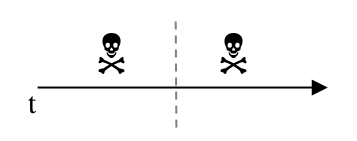
\includegraphics[scale=0.5]{figures/double-murder-knife-stabbing.png}
\captionof{figure}{Parts of a double murder event in a knife-stabbing scenario}\label{fig:parts-of-a-double-murder-event-in-a-knife-stabbing-scenario}
\end{figure}

Nonetheless, one could object that such an approach cannot account for situations such as a bomb scenario in which an intended explosion affected two victims leading to a double homicide. In such a case, quantification over temporally subsequent subevents is not possible since the explosion had an immediate effect and there was virtually no running time of the event. However, I believe there is no reason to assume that temporal chunks are the only possible parts that can constitute an event. Since events are complex peculiarities involving not only times, but also locations, in a bomb scenario described above it is still possible to differentiate between parts of an event in spatial terms. Consider the situation depicted in \figref{fig:parts-of-a-double-murder-event-in-a-bomb-scenario}. 

\begin{figure}[h!]
\centering
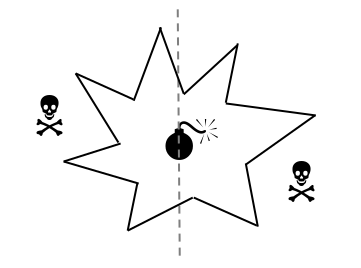
\includegraphics[scale=0.5]{figures/double-murder-bomb.png}
\captionof{figure}{Parts of a double murder event in a bomb scenario}\label{fig:parts-of-a-double-murder-event-in-a-bomb-scenario}
\end{figure}

Even with no temporally defined subevents it is quite straightforward that one could specify two areas within the space in which the explosion took place, as indicated by the dashed line. As a result, we obtain two parts of the murdering event each of which turns out to have the property of the whole and since individuals are in general assumed to occupy space, it should be possible to draw divisions like that with respect to any event.

Another way of explaining scenarios such as the one depicted in \figref{fig:parts-of-a-double-murder-event-in-a-bomb-scenario} would be to assume the uniqueness of roles condition on the individuation of events \citep[see][]{parsons1990events}. In such a case, the bomb explosion event can be described as consisting of two murdering subevents by distributing to different victims.

All things considered, it seems that the way of thinking about the meaning of multipliers I argue for can be easily extended to phrases involving reference to abstract peculiarities such as eventualities. Adopting a typal distinction between entities and events as typically assumed in standard Neo-Davidsonian frameworks \citep[e.g.,][]{carlson1984thematic,dowty1989semantic,parsons1990events}, along with the proposal that pluralities of events are obtained similarly to pluralities of entities \citep{bach1986algebra}, would simply require to ensure that the semantics of multipliers is general enough to cover both types of objects. In the next section, I will inspect yet another type of expression that is often modified by multipliers and does not necessarily denote concrete things. 

\subsection{Social roles}\label{sec:social-roles}

The final piece of data that appears to be problematic for the claim that multipliers are in fact subatomic quantifiers is constituted by phrases with nouns referring to social roles in examples such as those in \ref{ex:double-agent-polish}. 

\ex. Polish (NCP)\label{ex:double-agent-polish}
\ag. podwójny agent\\
double\textsc{.sg.m} agent\textsc{.m}\\
`double agent'\label{ex:double-agent-polish-agent}
\bg. podwójny mistrz\\
double\textsc{.sg.m} master\textsc{.m}\\
`double champion'\label{ex:double-agent-polish-champion}

Under ordinary circumstances, the phrase in \ref{ex:double-agent-polish-agent} does not refer to an individual who consists of two parts, e.g., Siamese twins working as spies, but rather they seem to involve a relationship between an individual and two other entities. To be an agent means to be an agent for some intelligence agency, i.e., one cannot be an agent without an employer for whom they spy. Likewise, \ref{ex:double-agent-polish-champion} refers to one person who is a champion in two disciplines. In both cases, the multiplier seems to quantify over entities denoted by the argument of the noun which at first blush is not expected given the previously discussed semantic behavior.

At this stage, it is not entirely clear how to integrate the ideas developed in this chapter with the treatment of examples such as those in \ref{ex:double-agent-polish}. However, a possible extension of the proposed view is to assume that nouns such as \textit{agent} involve some kind of an abstract association to entities related to denoted individuals, e.g., an association between agents and intelligence agencies, and that such an association is subject to part-whole relations. A promising perspective to pursue involves adopting the notion of roles into semantic theory \citep[see][]{sowa1984conceptual,steimann2000representation,zobel2017sensitivity,wagiel-toappear-slavic}. Intuitively, roles are functions or capacities of individuals, i.e., social constructs independent of the individuals that bear them. Crucially for our purposes, for an individual to bear a particular role, it must stand in a certain relationship to other individuals. Following \citet{zobel2017sensitivity}, one could distinguish between class nouns such as \textit{man}, i.e., properties of individuals of type $\langle e,t\rangle$, and role nouns such as \textit{agent} by adding a new type $r$ referring to roles and a shifting mechanism relating roles and individuals. Role nouns would then essentially denote properties of roles at type $\langle r,t\rangle$, but they could be shifted to refer to properties of entities as well. Within this view, multipliers would quantify over essential parts of roles rather than individuals and the whole phrase could then be shifted to refer to entities if required. This would account for the fact that expressions such as those in \ref{ex:double-agent-polish} denote individuals performing a complex role, i.e., individuals involved in activities and bearing responsibilities related to two distinct intelligence agencies. However, exploring the interaction between subatomic quantification and roles is rather challenging and goes beyond the scope of this study. Instead, in the next section I will return to the relationship between multipliers and cardinals.

\section{Multipliers vs. cardinals}\label{sec:multipliers-vs-cardinals}

As we saw in \sectref{sec:morphological-complexity-of-slavic-multipliers}, Slavic multipliers display morphological complexity, which suggests semantic compositionality. For instance, the Polish multiplier \textit{podwójny} `double' consists of the numeral root $\sqrt{\textit{dw}}$ corresponding to the number 2 present also in other types of numerical expressions, e.g., the cardinal \textit{dwa} `two', as well as additional morphemes including a special multiplicative circumfix \textit{po}$\rangle\dots\langle$\textit{n-}. This fact indicates that what multipliers and cardinals have in common is some sort of reference to integers. Though they both indicate that the number of quantified things equals 2, they differ in that they are devised to count entities of a distinct type. In particular, cardinals are semantically dedicated to count wholes. It is true that in Chapter \ref{ch:partitives-and-part-whole-structures} and \ref{ch:exploring-topological-sensitivity} we saw that they can be used in count explicit partitives in order to quantify over parts of objects, but notice that it is only possible when they modify a partitive word. In such a case, entities denoted by the whole partitive are treated as objects in their own right. Hence, the source of subatomic quantification is in fact the partitive, and the cardinal simply counts provided entities in their relative entirety. Bare cardinals can never access elements within a part-whole structure of a given entity. Rather, they always count entire objects in the denotation of a modified noun. On the other hand, multipliers are essentially subatomic quantifiers. They count parts of objects referred to by a modified nominal.

To better illustrate the claim introduced above, let us closely consider the contrasts between the truth conditions of the sentences involving numerical expressions in \ref{ex:cardinals-multipliers-crown-vault}. 

\ex. English (Guy Tabachnick, p.c.)\label{ex:cardinals-multipliers-crown-vault}
\a. There are two crowns in the vault.\label{ex:two-crown-vault}
\b. There are two parts of the crown in the vault.\label{ex:two-parts-crown-vault}
\b. There is a double crown in the vault.\label{ex:double-crown-vault}
\b. There are three double crowns in the vault.\label{two-double-crowns-crown-vault}

Under normal circumstances, there is no way the statement in \ref{ex:two-crown-vault} could be judged true if there were only two parts of a crown or crowns, e.g., an orb and a jewel, in the vault. The numeral phrase simply cannot be understood as referring to two parts instead of two entire objects.\footnote{Of course, what portion of an entity counts as an entire object is rather vague and might differ with respect to a particular predicate and a particular context. However, this is not at issue here.} In other words, cardinals are semantically devised to counting wholes. This is not in contradiction with the fact that in a sentence including a count explicit partitive construction as in \ref{ex:two-parts-crown-vault} the cardinal does count parts of a whole object. Consequently, \ref{ex:two-parts-crown-vault} would be true if there were only, say, an orb and a cross in the vault. Notice, however, that it is the partitive word that employs subatomic quantification. The cardinal here simply counts parts provided by the partitive construction as if they were considered objects in their own right. In other words, it does not operate on the part-whole structure of a given part. This contrasts with the meaning of \ref{ex:double-crown-vault} which would be true in a scenario where there were just one object in the vault. Crucially, however, that object would have to have two essential parts or, to put it differently, two parts having a property of being sort of a crown. Finally, the felicity of the sentence in \ref{two-double-crowns-crown-vault} shows that both types of quantification can co-occur within one phrase. Here, the multiplier triggers subatomic quantification constrained as discussed above, whereas the cardinal quantifies over wholes having the inner structure imposed by the multiplier. Consequently, the sentence would be true in a situation where in the vault there were three crowns such that each of them consisted of two self-sufficient parts. Notice that the relative order of the cardinal and multiplier as well as adjectival properties of the latter further suggest that subatomic quantification takes place first and only after the resulting wholes are counted.

The discussed contrast between cardinals and multipliers becomes even more salient if we consider what happens when the latter modify partitive words. Compare the examples in \ref{ex:two-double-part-adapter}. 

\ex. Polish\label{ex:two-double-part-adapter}
\ag. dwie części adaptera\\
two parts adapter\textsc{.gen}\\
`two parts of the adapter'\label{ex:two-part-adapter}
\bg. podwójna część adaptera\\
double part adapter\textsc{.gen}\\
`double part of the adapter'\label{ex:double-part-adapter}

We have already examined in detail count explicit partitives such as \ref{ex:two-part-adapter}, but let us now contemplate the meaning of an equivalent multiplier phrase such as \ref{ex:double-part-adapter}. Crucially, the multiplier quantifies over parts of a part of the adapter. The whole expression would be true of an entity that is an adapter part and consists of two comparable parts. Yet again, the multiplier employs quantification within the part-whole structure of a thing denoted by the nominal no matter what that thing is. Though such a use is for sure very rare, the phrase is definitely interpretable.\footnote{The example was actually found on a website of a producer of adapters with a picture of a described part. Source (accessed on 10th November 2020): \url{https://www.kstools.com/pl/produkty/narzedzia-specjalistyczne-do-samochodow-osobowych/silnik-system-paliwowy/czesci-pojedyncze/2159/podwojna-czesc-adaptera}.}

A natural example of a sentence with the discussed construction attested in the NCP is provided in \ref{ex:double-part-wall}.

\ex. Polish (NCP)\label{ex:double-part-wall}
\bg.[] Skrzynkę horyzontalną otwiera się podobnie jak podwójną część przedniej ścianki [\dots]\\
box\textsc{.acc} horizontal\textsc{.acc} opens \textsc{refl} similar how double\textsc{.acc} part\textsc{.acc} front\textsc{.gen} wall\textsc{.gen}\\
`The horizontal box can be opened similar to the double part of the front wall [\dots]'

I conclude that the purpose of cardinals is essentially to count whole entities in the extension of a modified nominal. If they modify a regular noun, they simply quantify over objects in its denotation. Similarly, if they appear in a count explicit partitive, they count provided parts in their entirety as if they were wholes. At the same time, natural language developed a special type of expression dedicated to numerical subatomic quantification, namely multipliers. Multipliers differ from cardinals in that they always count essential parts of objects denoted by a modified nominal be it a whole or a part. In other words, they are equipped to count parts within a whole. On the other hand, the two categories are similar in that although they typically count, sometimes they seem to measure. The quantificational properties of the two numerical expressions in question are summarized in  \tabref{tab:properties-of-cardinals-and-multipliers}.

    \begin{table}[h]
    \centering
\begin{tabular}{lcc}
\lsptoprule
                           & \textsc{cardinals} & \textsc{multipliers}  \\ \midrule
subatomic quantification   & *               & $\checked$    \\
quantification over wholes & $\checked$               & *    \\ \lspbottomrule
\end{tabular}
\caption{Properties of cardinals and multipliers}
\label{tab:properties-of-cardinals-and-multipliers}
\end{table}

This concludes the examination of some non-trivial properties of the neglected class of multipliers with respect to the issues concerning subatomic quantification. 

\section{Summary}\label{sec:summary-ch4}

In this chapter, I focused on a key topic concerning subatomic quantification. Specifically, I presented novel evidence demonstrating that in natural language there are numerical expressions devised for the purpose of quantification over parts, namely multipliers such as English \textit{double}. The fact that such lexical items are cross-linguistically widespread indicates the relevance of part-whole structures of singular objects for the interaction between parthood and quantification in natural language semantics. The morphological evidence from Slavic demonstrates that Polish, Czech, Russian, and Bosnian-Croatian-Serbian multipliers are formally complex expressions derived from numeral roots of corresponding cardinals. I argued that the morphological complexity of Slavic multipliers suggests semantic compositionality. 

Multipliers are sensitive to the internal part-whole structure of objects denoted by nouns they modify and involve quantification over cognitively most salient elements of those objects. Often, such elements are self-sufficient parts, i.e., entities that have a property comparable with the property of the whole. Sometimes, they are not self-sufficient but rather they are considered the most significant parts within the inner structure of an object. I generalized that multipliers count essential parts, i.e., parts perceived as crucial for an entity to be considered as having a particular property, with self-sufficient parts constituting a subset thereof. Moreover, I examined multiplier phrases involving mass terms. Interestingly, such expressions receive a portion interpretation and as such are countable. This fact indicates that multipliers either perform or require a mass-count shift in terms of packaging. Furthermore, I proposed how the view argued for here could be extended to cover cases of multiplier phrases involving other types of NPs, namely event nominals and role nouns. Incorporating abstract objects such as eventualities and roles into the ontology would allow us to capture the meaning of virtually all multiplier phrases in terms of one unified mechanism. Finally, I discussed how multipliers differ from cardinals. The crucial distinction between the two boils down to what type of entity they count in terms of part-whole structure. In particular, while cardinals always quantify over wholes, multipliers always count parts of a singular object which, similarly to complex entities or events they constitute, have themselves a property considered essential for an entity to fall in the denotation of a modified noun. 

This chapter concludes the empirical part of this book. The most important insights could be summarized as follows. First, singulars and plurals share a unified part-whole structure. Second, natural language is sensitive to topological relations holding between parts of entities in the denotations of nominal expressions and allows for quantification at the subatomic level. Third, only entities that are perceived as constituting integrated wholes are conceptualized as countable. Finally, though different types of numerical expressions specialize in quantification either over wholes or over parts, the underlying mechanism is the same. In the next chapter, I will introduce the conceptual background that will serve as an informal notional basis for a formal account for subatomic quantification.
